\newpage

%%%%%%%%%%%%%%%%%%%%%%%%%%%%%%%%%%%%%%%%%%%%%%%%%%%%%%%%%%%%%%%%%%%%%%%%%%%%%%%%%%%%%%%
%%%%%%%%%%%%%%%%%%%%%%%%%%%%%%%%%%%%%%%%%%%%%%%%%%%%%%%%%%%%%%%%%%%%%%%%%%%%%%%%%%%%%%%
%%%%%%%%%%%%%%%%%%%%%%%%%%%%%%%%%%%%%%%%%%%%%%%%%%%%%%%%%%%%%%%%%%%%%%%%%%%%%%%%%%%%%%%
\section{Regressão logística polinomial com MSE de $f_{\VECTOR{c}}(\VECTOR{x}):~\mathbb{R}^{N} \rightarrow \mathbb{R}$}

\index{Regressão!Logística polinomial $f_{\VECTOR{c}}(\VECTOR{x}):~\mathbb{R}^{N} \rightarrow \mathbb{R}$}
\index{Polinômio multivariante}

\begin{theorem}[Classificação de dados em $\mathbb{R}^{N}$:]\label{theo:reglogrnr1poly:1}
~\\
\noindent
\begin{minipage}{0.45\textwidth}
\centering
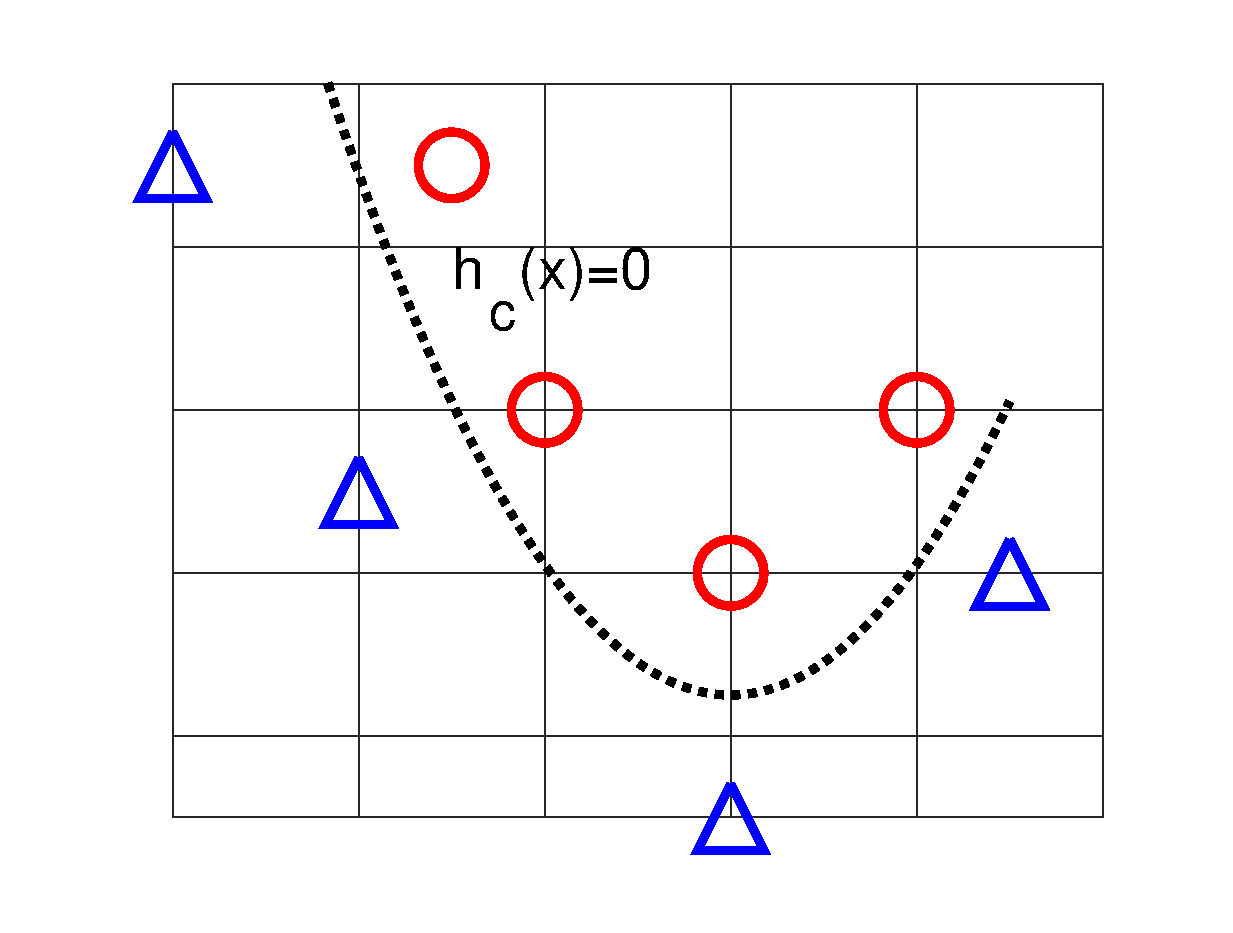
\includegraphics[width=0.95\linewidth]{chapters/classificacao/mfiles/reglogrnr1poly/reglogrnr1poly.eps} 
\end{minipage}
\begin{minipage}{0.55\textwidth}
Dados, um conjunto de $L$ pontos
$\VECTOR{x}_l$ $\in \mathbb{R}^{N}$, $1\leq l \leq L$,
repartidos em dois grupos etiquetados com os símbolos $\bigtriangleup$ e $\bigcirc$,
não separáveis por um hiperplano  em $\mathbb{R}^{N}$.
Se desejamos criar um classificador mediante 
a função  $f_{\VECTOR{c}}:\mathbb{R}^{N} \rightarrow \mathbb{R}$,
com domínio $\VECTOR{x} \in \mathbb{R}^{N}$, contradomínio $y \in \mathbb{R}$ e 
parâmetros agrupados no vetor $\VECTOR{c}$,
como definido na Eq. (\ref{eq:reglogrnr1poly:1}),
\begin{equation}\label{eq:reglogrnr1poly:1}
y\equiv f_{\VECTOR{c}}(\VECTOR{x})= \frac{1}{1+e^{-h_{\VECTOR{c}}(\VECTOR{x})}},
\quad h_{\VECTOR{c}}(\VECTOR{x})=\VECTOR{a}_M(\VECTOR{x})\VECTOR{c},
\end{equation}
\end{minipage}
ou seu equivalente: $logit(y)=h_{\VECTOR{c}}(\VECTOR{x})$,
sendo $h_{\VECTOR{c}}(\VECTOR{x})$ um polinômio multivariante de grau total $M$ 
\cite[pp. 47]{geddes2007algorithms} \cite[pp. 108]{zippel2012effective}
com coeficientes agrupados no vetor $\VECTOR{c}$.
Podemos atribuir a cada valor $\VECTOR{x}_l$ uma etiqueta $y_l\in \{A,1-A\}$, 
$A$ para $\bigtriangleup$ e  $1-A$ para $\bigcirc$,
onde $0<A\ll 0.5$ é escolhido por nós,
e afirmar que o vetor $\VECTOR{c}= \VECTOR{\hat{c}}$,
que minimiza o erro quadrático médio\footnote{Do inglês ``mean square error'' com siglas $MSE$.} $e(\VECTOR{c})$,
\begin{equation}\label{eq:reglogrnr1poly:1e}
e(\VECTOR{c}) =  \frac{1}{L}\sum_{l=1}^{L} w_l||h_{\VECTOR{c}}(\VECTOR{x}_l)-logit(y_l)||^2,
\end{equation}
pode ser achado mediante a Eq. (\ref{eq:reglogrnr1poly:2}).
Os erros de cada amostra são ponderados com os pesos $w_l \in \mathbb{R}_+$ e
agrupados na matriz  $\MATRIX{W}=\funcdiag \left( \left[w_1,~ w_2,~ ...,~ w_L \right]^{\transpose} \right) $;
\begin{equation}\label{eq:reglogrnr1poly:2}
\VECTOR{\hat{c}} =  \left[ \MATRIX{A}^{\transpose} \MATRIX{W}\MATRIX{A}\right]^{-1} \MATRIX{A}^{\transpose} \MATRIX{W}\VECTOR{z},
\quad
\MATRIX{A}=
\begin{bmatrix}
a_M(\VECTOR{x}_1)\\
a_M(\VECTOR{x}_2)\\
%\vdots\\
%a_M(\VECTOR{x}_l)\\
\vdots\\
a_M(\VECTOR{x}_L)\\ 
\end{bmatrix},
\quad
\VECTOR{z}=
\begin{bmatrix}
logit(y_1)  \\
logit(y_2)  \\
%\vdots  \\
%logit(y_l)  \\
\vdots \\
logit(y_L) \\
\end{bmatrix},
\end{equation}
\begin{equation}\label{eq:reglogrnr1poly:3}
\VECTOR{a}(\VECTOR{x})=
\begin{bmatrix}
\VECTOR{b}_0(\VECTOR{x}) &
\VECTOR{b}_1(\VECTOR{x}) &
\hdots &
\VECTOR{b}_m(\VECTOR{x}) &
\hdots &
\VECTOR{b}_M(\VECTOR{x}) 
\end{bmatrix},
\end{equation}
\begin{equation}\label{eq:reglogrnr1poly:4}
\VECTOR{b}_0(\VECTOR{x})=
\begin{bmatrix}
1 
\end{bmatrix},
\quad 
\VECTOR{b}_1(\VECTOR{x})=
\begin{bmatrix}
x_1 & x_2 & ... &  x_N
\end{bmatrix},
\quad 
\VECTOR{b}_m(\VECTOR{x})=
{\bigcup\limits_{\alpha_1+\alpha_2+...+\alpha_N=m}^{\rightarrow}}{x_1^{\alpha_1} x_2^{\alpha_2} ... x_N^{\alpha_N}} .
\end{equation}
$\VECTOR{b}_m(\VECTOR{x})$ representa um vetor linha com elementos $x_1^{\alpha_1} x_2^{\alpha_2} ... x_N^{\alpha_N}$
de modo que em cada elemento se cumpre que $\alpha_1+\alpha_2+...+\alpha_N=m$,
sendo que $\alpha_n \in \mathbb{N}$.
\end{theorem}

\begin{tcbattention}
\begin{itemize}
\item Dado que a função de classificação $f_{\VECTOR{c}}(\VECTOR{x})$ vai entre $0$ e $1$,
podemos reinterpretar este valor como se fosse uma probabilidade;
neste caso, $f_{\VECTOR{c}}(\VECTOR{x})$ representa a probabilidade de que um ponto $\VECTOR{x}$
pertença ao grupo $\bigcirc$.
\item O limiar de classificação na função $f_{\VECTOR{c}}(\VECTOR{x})$ está no hiperplano $h_{\VECTOR{c}}(\VECTOR{x})=0$.
%provocando nestos pontos um $f_{\VECTOR{c}}(\VECTOR{x})=0.5$.
\item A ordem dos elementos do vetor $\VECTOR{a}_M(\VECTOR{x})$ podem ser alterados,
isto só modificará a posição dos elementos no vetor $\VECTOR{c}$.
\end{itemize}
\end{tcbattention}


\begin{example}[Polinômios multivariante:]\label{ex:theo:reglogrnr1poly:multinomio}~\\
\begin{itemize}
\item Polinômio univariado de grau total 2: 
$P_{\VECTOR{c}}(x)=c_1 + c_2 x + c_3 x^2$.
\begin{equation}
\VECTOR{b}_0(x)=[1],
\quad 
\VECTOR{b}_1(x)=[x],
\quad 
\VECTOR{b}_2(x)=[x^2].
\end{equation}
\item Polinômio bivariado de grau total 2: 
$P_{\VECTOR{c}}(\VECTOR{x})=c_1 + c_2 x_1 + c_3 x_2 + c_4 x_1^2 + c_5 x_1 x_2+ c_6 x_2^2$.
\begin{equation}
\VECTOR{b}_0(\VECTOR{x})=
\begin{bmatrix}
1
\end{bmatrix},
\quad 
\VECTOR{b}_1(\VECTOR{x})=
\begin{bmatrix}
x_1 & x_2
\end{bmatrix},
\quad 
\VECTOR{b}_2(\VECTOR{x})=
\begin{bmatrix}
x_1^2 & x_2^2 & x_1x_2
\end{bmatrix}.
\end{equation}
\item Polinômio trivariado de grau total 2: 
$P_{\VECTOR{c}}(\VECTOR{x})=c_1 + 
c_2 x_1 + c_3 x_2 + c_4 x_3 + 
c_5 x_1^2 + c_6 x_2^2 + c_7 x_3^2 + c_8 x_1 x_2+ c_9 x_1 x_3 + c_{10} x_2 x_3$.
\begin{equation}\label{eq:b0b1b2}
\VECTOR{b}_0(\VECTOR{x})=
\begin{bmatrix}
1
\end{bmatrix},
\quad 
\VECTOR{b}_1(\VECTOR{x})=
\begin{bmatrix}
x_1 & x_2 & x_3
\end{bmatrix},
\quad 
\VECTOR{b}_2(\VECTOR{x})=
\begin{bmatrix}
x_1^2 & x_2^2 & x_3^2 & x_1x_2 & x_1x_3 & x_2x_3
\end{bmatrix}.
\end{equation}
\end{itemize}
\end{example}

\index{Multiset}
\index{Multiconjunto}
\begin{theorem}[Número de elementos de $\VECTOR{b}_m(\VECTOR{x})$:]\label{theo:reglogrnr1poly:bm}
Dada uma função vetorial $\VECTOR{b}_m(\VECTOR{x})$ de parâmetro $\VECTOR{x}\in \mathbb{R}^{N}$,
a quantidade de elementos $L_{\VECTOR{b}}(N,m)$ do vetor $\VECTOR{b}_m(\VECTOR{x})$ pode ser calculado com 
\begin{equation}
L_{\VECTOR{b}}(N,m)=\frac{N(N+1)(N+2)...(N+m-1)}{m!}=\binom{N+m-1}{m}.
\end{equation}
\textbf{Prova:} $L_{\VECTOR{b}}(N,m)$ representa o número de combinações (grupos ou multiconjuntos) com repetição,
onde  cada grupo tem $m$ elementos,
escolhidos de um total de $N$ elementos, quando a ordem de escolha não importa, 
e os elementos podem ser escolhidos mais de uma vez em cada grupo.
\end{theorem}

\begin{table}[h!]
\centering
\begin{tabular}{|c||c|c|c|c|} 
 \hline
~        & $\VECTOR{b}_0(\VECTOR{x})$ & $\VECTOR{b}_1(\VECTOR{x})$ & $\VECTOR{b}_2(\VECTOR{x})$ & $\VECTOR{b}_3(\VECTOR{x})$  \\ \hline
$L_{\VECTOR{b}}(N,m)$ & $1$ & $N$ & $\frac{N(N+1)}{2}$ & $\frac{N(N+1)(N+2)}{3!}$\\ \hline
\end{tabular}
\caption{Número de elementos de $\VECTOR{b}_m(\VECTOR{x})$.}
\label{table:theo:reglogrnr1poly:bm}
\end{table}

%%%%%%%%%%%%%%%%%%%%%%%%%%%%%%%%%%%%%%%%%%%%%%%%%%%%%%%%%%%%%%%%%%%%%%%%%%%%%%%%
\subsection{Exemplos de classificação com uma função
$f_{\VECTOR{c}}(\VECTOR{x}):~\mathbb{R}^N \rightarrow \mathbb{R}$ }

\begin{example}\label{ex:theo:reglogrnr1poly}
Conhecidas as $L=10$ amostras $\VECTOR{x}_l$ e seus respetivos grupos indicados pelos símbolos $\bigtriangleup$ e $\bigcirc$, 
mostrados na Tabela \ref{table:theo:reglogrnr1poly:xn},
achar o classificador $f_{\VECTOR{c}}(\VECTOR{x})$ que usa um polinômio multivariante $h_{\VECTOR{c}}(x)$
de grau total $M=2$, 
que gere o menor erro $e(\VECTOR{c}) =  \frac{1}{L}\sum_{l=1}^{L} ||h_{\VECTOR{c}}(\VECTOR{x}_l)-logit(y_l)||^2$.
\end{example}


\begin{table}[h!]
\centering
\begin{tabular}{|c||c|c|c|c|c||c|c|c|c|c||} 
 \hline
$l$            & 1 & 2 & 3 & 4 & 5 & 6 & 7 & 8 & 9 & 10 \\ \hline \hline
$\VECTOR{x}_l$ & 1 & 1 & 2 & 4 & 5 & 2 & 2 & 3 & 5 & 6 \\ 
~              & 5 & 4 & 2 & 1 & 1 & 6 & 5 & 3 & 2 & 2 \\ \hline
$\VECTOR{y}_l$ & $\bigtriangleup$ & $\bigtriangleup$ & $\bigtriangleup$ & $\bigtriangleup$ & $\bigtriangleup$ 
      & $\bigcirc$ & $\bigcirc$ & $\bigcirc$ & $\bigcirc$ & $\bigcirc$\\ \hline
\end{tabular}
\caption{Valores $\VECTOR{x}_l$.}
\label{table:theo:reglogrnr1poly:xn}
\end{table}


\begin{SolutionT}[Relativa ao Exemplo \ref{ex:theo:reglogrnr1poly}:]\label{sol:theo:reglogrnr1poly:s1}
Para obter o vetor de parâmetros $\VECTOR{c}=\VECTOR{\hat{c}}$ da função $f_{\VECTOR{c}}(\VECTOR{x})$, 
que gere o menor erro $e(\VECTOR{c}) = \frac{1}{L} \sum_{l=1}^{L} ||h_{\VECTOR{c}}(\VECTOR{x}_l)-logit(y_l)||^2$
com os $L=10$ dados $\VECTOR{x}_l$ da Tabela \ref{table:theo:reglogrnr1poly:xn},
usamos as Eqs. (\ref{eq:b0b1b2}) e  (\ref{eq:reglogrnr1poly:2}) onde escolhemos $w_l=1$ e valores $y_l \in \{0.1,~ 0.9\}$,
$0.1$ para $\bigtriangleup$ e $0.9$ para $\bigcirc$, 
obtendo um vetor 
\begin{equation}
\VECTOR{\hat{c}}=[-11.71919\quad 2.49938\quad 2.49938\quad -0.30282\quad -0.30282\quad 0.50579]^{\transpose}.
\end{equation}
Assim, podemos representar a função $f_{\VECTOR{c}}(\VECTOR{x})$ que classifica os dados $\VECTOR{x}_l$, 
como é mostrado na Figura \ref{fig:theo:reglogrnr1poly:xn:s1},
\begin{equation}
f_{\VECTOR{c}}(\VECTOR{x})= \frac{1}{1+e^{-h_{\VECTOR{c}}(\VECTOR{x})}},
\quad
\begin{array}{lll}
h_{\VECTOR{c}}(\VECTOR{x}) & = & -11.71919\\
                         ~ & ~ & +2.49938 x_1 +2.49938 x_2 \\
                         ~ & ~ & -0.30282 x_1^2 -0.30282  x_2^2 + 0.50579 x_1 x_2.\\
\end{array}
\end{equation}
É interessante ressaltar que para um valor $A=0.1$ a pendente na mudança de classificação é pouco definida,
com limiares de classificação na superfície $h_{\VECTOR{c}}(\VECTOR{x})=0$.
\end{SolutionT}

\begin{figure}[!h]
    \begin{subfigure}[b]{0.45\textwidth}
        \centering
        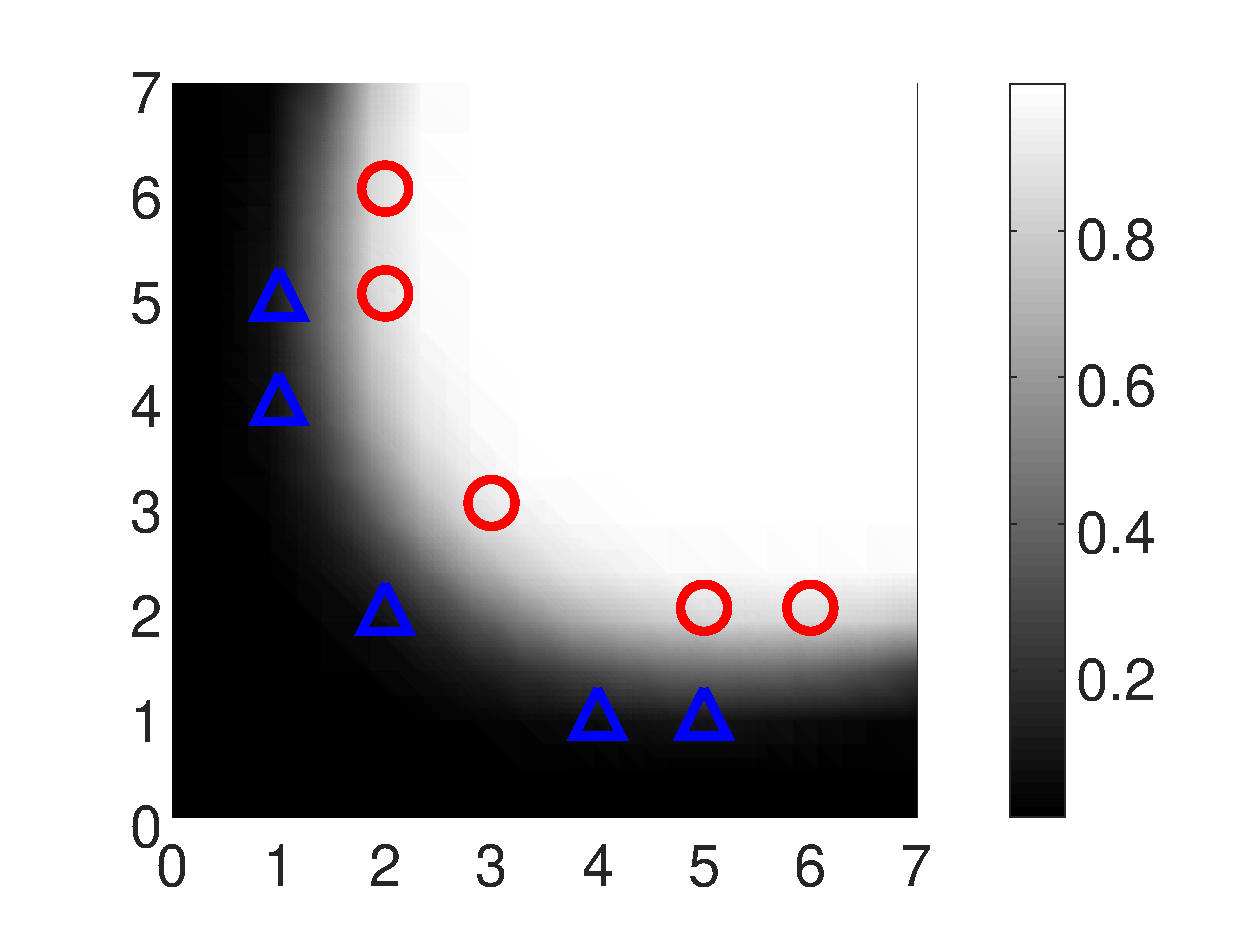
\includegraphics[width=\textwidth]{chapters/classificacao/mfiles/reglogrnr1poly/ex1s1-reglogrnr1poly.eps}
        \caption{Gráfico da classificação usando $y_l \in \{0.1,~ 0.9\}$.}
        \label{fig:theo:reglogrnr1poly:xn:s1}
    \end{subfigure}
    \hfill
    \begin{subfigure}[b]{0.45\textwidth}
        \centering
        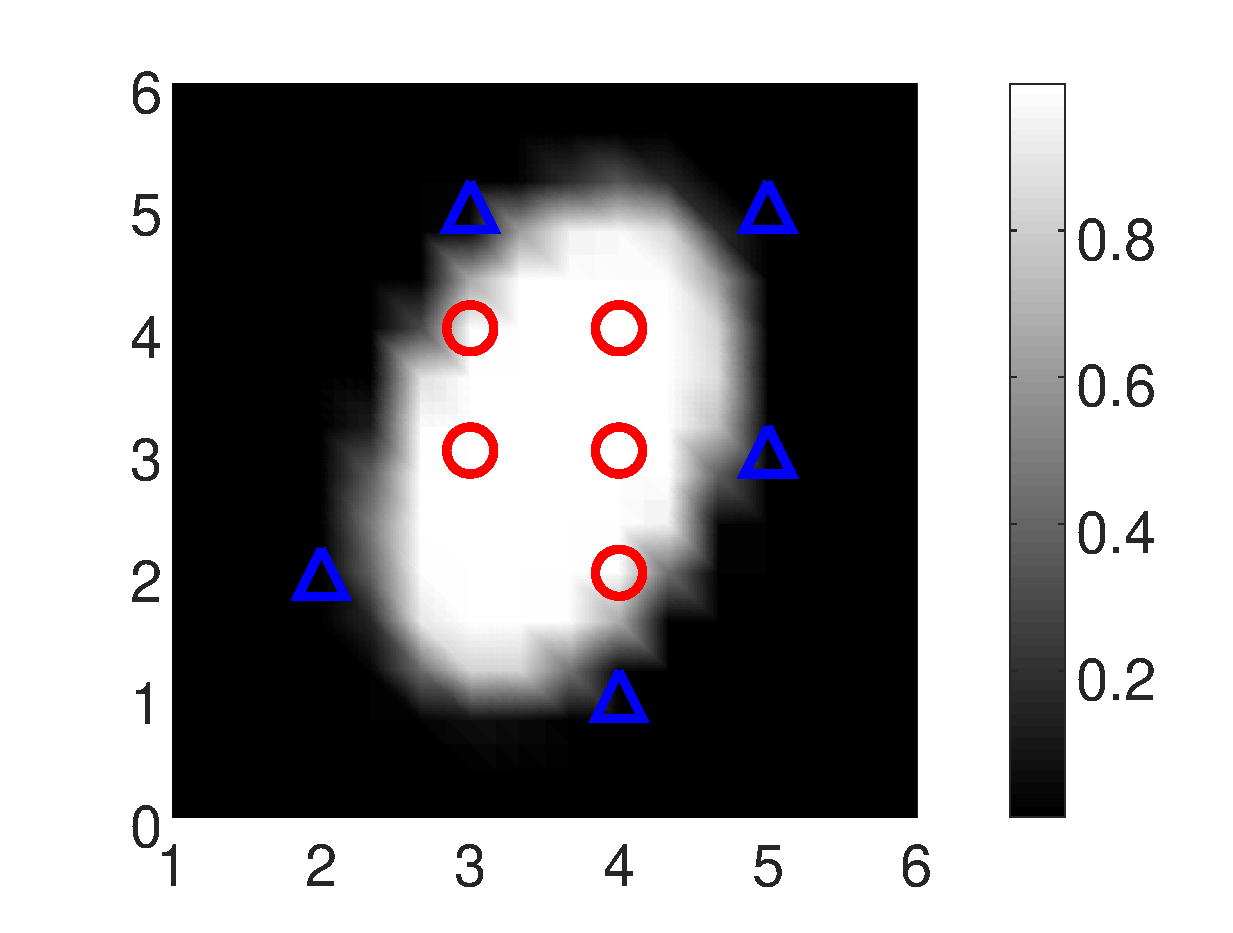
\includegraphics[width=\textwidth]{chapters/classificacao/mfiles/reglogrnr1poly/ex1s2-reglogrnr1poly.eps}
        \caption{Gráfico da classificação usando $y_l \in \{0.001,~ 0.999\}$.}
        \label{fig:theo:reglogrnr1poly:xn:s2}
    \end{subfigure}
    \caption{Classificação usando a função $f_{\VECTOR{c}}(\VECTOR{x})$.}
    \label{fig:theo:reglogrnr1poly:xn}
\end{figure}


\begin{SolutionT}[Relativa ao Exemplo \ref{ex:theo:reglogrnr1poly}:]\label{sol:theo:reglogrnr1poly:s2}
Para obter o vetor de parâmetros $\VECTOR{c}=\VECTOR{\hat{c}}$ da função $f_{\VECTOR{c}}(\VECTOR{x})$, 
que gere o menor erro $e(\VECTOR{c}) = \frac{1}{L} \sum_{l=1}^{L} ||h_{\VECTOR{c}}(\VECTOR{x}_l)-logit(y_l)||^2$
com os $L=10$ dados $\VECTOR{x}_l$ da Tabela \ref{table:theo:reglogrnr1poly:xn},
usamos as Eqs. (\ref{eq:b0b1b2}) e  (\ref{eq:reglogrnr1poly:2}) 
onde escolhemos $w_l=1$ e valores $y_l \in \{0.001,~ 0.999\}$,
$0.001$ para $\bigtriangleup$ e $0.999$ para $\bigcirc$, 
obtendo um vetor 
\begin{equation}
\VECTOR{\hat{c}}=[-36.83809\quad 7.85656\quad 7.85656\quad -0.95187\quad -0.95187\quad 1.58990]^{\transpose}.                  
\end{equation}
Assim, podemos representar a função $f_{\VECTOR{c}}(\VECTOR{x})$ que classifica os dados $\VECTOR{x}_l$, 
como é mostrado na Figura \ref{fig:theo:reglogrnr1poly:xn:s2},
\begin{equation}
f_{\VECTOR{c}}(\VECTOR{x})= \frac{1}{1+e^{-h_{\VECTOR{c}}(\VECTOR{x})}},
\quad
\begin{array}{lll}
h_{\VECTOR{c}}(\VECTOR{x}) & = & -36.83809\\
                         ~ & ~ & +7.85656 x_1 +7.85656 x_2 \\
                         ~ & ~ & -0.95187 x_1^2 -0.95187  x_2^2 + 1.58990 x_1 x_2.\\
\end{array}
\end{equation}
É interessante ressaltar que para um valor $A=0.001$ a pendente na mudança de classificação está bem definida,
com limiares de classificação na superfície $h_{\VECTOR{c}}(\VECTOR{x})=0$.
\end{SolutionT}
